\documentclass[ProjectUYA]{subfiles}
% WARNING: AuCTeX local variables only get reset when file is loaded
% and differ between this file and BufferStockTheory.tex
% so must re-load whichever file you want to compile with C-x C-v

% WARNING: Different AucTeX execution depending on whether
% 0. Being compiled as standalone document
% * Compile main once
% * Then compile this one
% * Keep compiling until nothing changes
% 0. Being compiled as subfile of main document
% * Just compile main document repeatedly

% LaTeX path to the root directory of the current project, from the directory in which this file resides
% and path to econtexPaths which defines the rest of the paths like \FigDir
\providecommand{\econtexRoot}{}\renewcommand{\econtexRoot}{.}
\providecommand{\econtexPaths}{}\renewcommand{\econtexPaths}{\econtexRoot/Resources/econtexPaths}
% The \commands below are required to allow sharing of the same base code via Github between TeXLive on a local machine and Overleaf (which is a proxy for "a standard distribution of LaTeX").  This is an ugly solution to the requirement that custom LaTeX packages be accessible, and that Overleaf prohibits symbolic links
\providecommand{\econtex}{\econtexRoot/Resources/texmf-local/tex/latex/econtex}
\providecommand{\econtexSetup}{\econtexRoot/Resources/texmf-local/tex/latex/econtexSetup}
\providecommand{\econtexShortcuts}{\econtexRoot/Resources/texmf-local/tex/latex/econtexShortcuts}
\providecommand{\econtexBibMake}{\econtexRoot/Resources/texmf-local/tex/latex/econtexBibMake}
\providecommand{\econtexBibStyle}{\econtexRoot/Resources/texmf-local/bibtex/bst/econtex}
\providecommand{\econtexBib}{economics}
\providecommand{\notes}{\econtexRoot/Resources/texmf-local/tex/latex/handout}
\providecommand{\handoutSetup}{\econtexRoot/Resources/texmf-local/tex/latex/handoutSetup}
\providecommand{\handoutShortcuts}{\econtexRoot/Resources/texmf-local/tex/latex/handoutShortcuts}
\providecommand{\handoutBibMake}{\econtexRoot/Resources/texmf-local/tex/latex/handoutBibMake}
\providecommand{\handoutBibStyle}{\econtexRoot/Resources/texmf-local/bibtex/bst/handout}

\providecommand{\FigDir}{\econtexRoot/Figures}
\providecommand{\CodeDir}{\econtexRoot/Code}
\providecommand{\DataDir}{\econtexRoot/Data}
\providecommand{\SlideDir}{\econtexRoot/Slides}
\providecommand{\TableDir}{\econtexRoot/Tables}
\providecommand{\ApndxDir}{\econtexRoot/Appendices}

\providecommand{\ResourcesDir}{\econtexRoot/Resources}
\providecommand{\rootFromOut}{..} % Path back to root directory from output-directory
\providecommand{\LaTeXGenerated}{\econtexRoot/LaTeX} % Put generated files in subdirectory
\providecommand{\econtexPaths}{\econtexRoot/Resources/econtexPaths}
\providecommand{\LaTeXInputs}{\econtexRoot/Resources/LaTeXInputs}
\providecommand{\LtxDir}{LaTeX/}
\providecommand{\EqDir}{Equations} % Put generated files in subdirectory


\onlyinsubfile{% https://tex.stackexchange.com/questions/463699/proper-reference-numbers-with-subfiles
    \csname @ifpackageloaded\endcsname{xr-hyper}{%
      \externaldocument{\econtexRoot/BufferStockTheory}% xr-hyper in use; optional argument for url of main.pdf for hyperlinks
    }{%
      \externaldocument{\econtexRoot/BufferStockTheory}% xr in use
    }%
    \renewcommand\labelprefix{}%
    % Initialize the counters via the labels belonging to the main document:
    \setcounter{equation}{\numexpr\getrefnumber{\labelprefix eq:Dummy}\relax}% eq:Dummy is the last number used for an equation in the main text; start counting up from there
}


\onlyinsubfile{\externaldocument{ProjectUYA}} % Get xrefs -- esp to appendix -- from main file; only works properly if main file has already been compiled;

\begin{document}


% Attempted to make all lines used for Web version contain {Web} (or version with only single curly brace at end) so can be removed with sed
\providecommand{\versn}{pdf} % Version; like, web or pdf or journal submission
\ifthenelse{\boolean{Web}}{    % {Web}
  \renewcommand{\versn}{Web}     % Too hard to figure out passing -output-directory through make4ht through htlatex, so web version is compiled with junk files in main directory
  \renewcommand{\rootFromOut}{.} % {Web}
}{}  % {Web}

% Tiny info header at top to track git commit
%\hfill{\tiny \jobname~\versn~\today~{at} \DTMcurrenttime, \input{\ResourcesDir/.git-source-commit}~~\input{\ResourcesDir/.git-public-commit}}

\title{Pension reforms in Kazakhstan using an OLG model}

\author{Uldana Abdikarim\authNum}

\keywords{OLG, pension reforms}




\maketitle
\hypertarget{abstract}{}
\begin{abstract}
  The aim of this paper is to study the effects of recently introduced pension reform in Kazakhstan on the welfare of the country. The effect of increase in mandatory retirement age for women from 58 to 63 is of primary interest of the paper. In order to achieve this goal, I propose 4-period OLG model with three main sectors of the economy and a fully-funded pension system.
\end{abstract}





{\titlepagefinish}


\section{Introduction}\label{sec:intro}
Financial sustainability of pension systems is one the primary concerns of the governments along with the effectiveness of these systems in terms of providing social security assistance to population. Therefore, different government reforms are conducted in response to changing demographics, changes in employment, economic and political shocks. Kazakhstan is among numerous countries that implemented new social security policies in the last twenty years. The country inherited a generous pension system from the Soviet Union with high replacement rate and early retirement age. However, independent Kazakhstan could not continue employing such a system due to economic instability, decrease in formal employment and changing demographics. As a result, Kazakhstan attempted several pension reforms to establish a pension system sustainable in the long term. 

The first major pension reform took place in 1998, which replaced the old pay-as-you-go system with a fully funded pension system, which required workers to make compulsory 10\% contribution to their individual accounts. Under the new reform, only those individuals, who worked at least 6 month prior to 1998 were eligible for pension benefits of old PAYG system. In 2013, another major reform in the pension system was introduced. According to the new law, all pension contributions were to be managed by the Unified Accumulative Pension Fund, replacing private pension funds, asset management companies and the state fund. Moreover, mandatory retirement age for women was increased from 58 to 63. This particular aspect of the reform was negatively received by the population \cite{maltseva}. As a result, the government decided to gradually increase the mandatory retirement age for women by six month each year starting from 2018. In order to provide sufficient replacement rate for the retired population, the government planned to introduce changes in the pension system starting from 2020. The change would have required employers to contribute 5\% of the wages into the individual accounts on top of existing 10\% employee contributions. However, the initiative has been recently postponed until 2023.

\begin{figure}[ht]
  \centerline{
    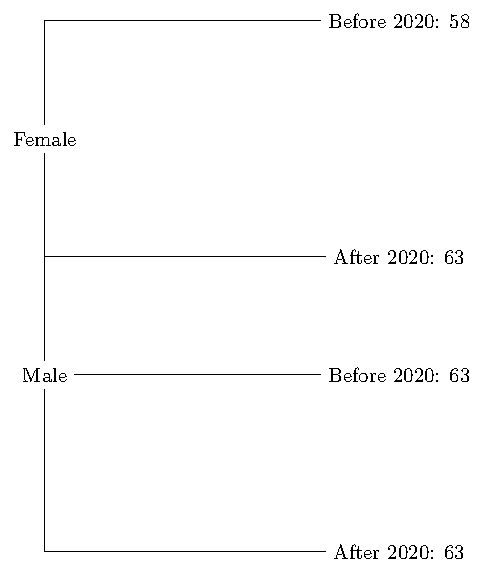
\includegraphics[width=6.0in]{\FigDir/Pension-age}
}
  \caption{Male and Female retirement age} \label{fig:Timeline}

\end{figure}


\newpage
The welfare effects of the proposed pension reforms are of primary interest of this paper. Increase in mandatory retirement age of women from 58 to 63 and introduction of 5\% employer contribution to the individual pension accounts are analyzed in the framework of fully-funded pension system using OLG model. First, brief overview of the existing literature on OLG models and social security systems will be presented. Then, the baseline OLG model will be described. Eventual goal is to do the policy simulations of the proposed pensions reforms. 


\section{Literature Review}
\cite{diamond} pioneered the use of OLG model in analyzing economic questions, by using two-generation model for the analysis in monetary economics. Since then, more complicated models with more generations have been introduced by the scholars to study wide variety of economic issues. The question of the effectiveness of social security reforms has been addressed by multitude of studies. Auerbach and Kotlikof \cite{auerbach} develop 55 generations OLG model to study the social security system along with other government reforms. The models were extended by the economists to study the various aspects of social security reforms. OLG models are used to compare the effects of fully-funded and PAYG pension systems on different economic indicators such as hours worked, earnings, savings, etc. \cite{buyse} and to study the effects of population aging on an economy \cite{muto}, \cite{heijdra}. A more recent research on the US social security system found that transitioning from PAYG system to a fully-funded one would substantially improve the welfare of all cohorts of households in the model \cite{mcgrattan}.

The effects of changes in mandatory retirement age, pension contribution rates, and pension benefits under a certain pension system on GDP growth, life-time utility of the consumers, and labor supply have been studied using OLG models. Policy simulation results suggest that increasing retirement age lead to higher GDP growth in both short-run and long-run \cite{cournede}. \cite{hsu} analyzes similar pension reforms under PAYG system with four-sector and sixty-generation economy.The author finds that although increasing retirement age lowers life-time utility for current generations, it results in higher life-time utility for future generations. Similarly, increase in contribution rates result in higher GDP growth rate. \cite{karam} find that the positive effect of the higher contribution rates on GDP growth is weaker compared to the effect of increased retirement age. \cite{hsu} also finds that increase in contribution rate harms government budgetary condition, but leads to higher GDP growth rate.

\cite{imroh}, using microdata from US for calibration, found that increase in retirement age by 2 years leads to higher labor supply and capital stock. While this paper examines the similar question of effects of increase in retirement age, it uses significantly simplified model compared to the one build by Imrohoroglu and Kitao. Their model allows the agents to decide when to retire, making the claim for pension benefits endogenous. Moreover, unlike the model build in this paper, it includes health risks, probability of mortality, and medical expenditures.


\section{Model}
This paper's main goal is to analyze the effect of increase in mandatory retirement age for women from 58 to 63 on hours worked, income and welfare under the fully funded pension system using the OLG model.

Until 2018, male and female retirement ages were 63 and 58 for men and women, respectively. Life expectancy for men and women in Kazakhstan are 69 and 77, respectively. Starting from 2018, female retirement age has started to increase by 6 months each year. In the baseline model, retirement age for women is set to be 58. 

 Let us start with a description of the different agents in the model. In global terms, the model presented is a perfect-foresight, 4 period-lived household overlapping generations model. A unit measure 
 of households are born in each period and each individual lives for four periods. Households supply labor in every period and choose how much to consume and how much to save through investment. A unit measure of identical, perfectly competitive firms rent investment capital from households and hire labor from households. 


 Two comments are in order:
 	\begin{enumerate}
 		\item  The assumption that individuals live for 4 periods is meant to capture each of the \emph{significant} lapses of time across the life-time of the household. In particular, the four different periods in this economy face are fundamentally different because of the different budget constraints that the households face in each of the periods. This is a simplifying assumption that attempts to model the 56 years of the average working life-span of a Kazakhstani household. This assumption is meant to explain as quickly as possible the main features of the model. 
 		\item To simplify the exposition here, I will assume that households are the owners of the capital endowment in the economy, and are, therefore, in charge of the investment decisions in the economy. 
 	\end{enumerate}

 In the next sections, I will describe each of the components of the model.

 \subsection{Households}

 A unit measure of identical households are born each period and live for four periods. Let the age of a household be indexed by $s\in\{1,2,3,4\}.$ Each household is composed of a female and a male. Households get paid wage rate $w_t$ for the labor they offer to firms market and a net return\footnote{gross return minus depreciation $\sigma$} $r_t$. In general, an age-$s$ household
 faces the following\footnote{Note that the budget constraints are written in the most general way possible to make it easier to extend the model. Later we will not have only 4 periods but 56, but the budget constraints will conform to four general time lapses, as described before. } budget constraints:
 

 	 \begin{align}
 	c_{s,t+s-1} + k_{s+1,t+s} &= (1-\tau_b)w_t (2-\ell_{s,t}^m - \ell_{s,t}^f) + r_{t+s-1}k_{s,t+s-1} & \forall t\text{ and for $s=1$} \\
 	c_{s,t+s-1} + k_{s+1,t+s} &= b_{t+s-1}^f+(1-\tau_b)w_t (1-\ell_{s,t}^m ) + r_{t+s-1}k_{s,t+s-1} & \forall t\text{ and for $s=2$} \\
 	c_{s,t+s-1} + k_{s+1,t+s} &= b_{t+s-1}^f+ b_{t+s-1}^m  + r_{t+s-1}k_{s,t+s-1} & \forall t\text{ and for $s=3$} \\
 	c_{s,t+s-1} + k_{s+1,t+s} &= b_{t+s-1}^f + r_{t+s-1}k_{s,t+s-1} & \forall t\text{ and for $s=4$}
 \end{align}


Household's are composed of a male and a female, in the periods that they are alive, each sex is endowed with one unit of leisure. At age $s=1$, both of them choose how much leisure to have, i.e., they choose how much labor to supply to the market for every $t$. At age $s=2$ males choose again how much leisure to have for every $t$; but at age $s=3$ males retire so that  $\ell_{s,t}^m=1$ for every $t$; finally,  At age $s=4$ $\ell_{4,t}=0$ for every $t$, since males have died at this point. On the other hand, females are retired from age 2 onwards, so that for $s=2,3,4$, we have that $\ell_{s,t}^f=1$ for every $t.$ The household's supply of labor, by sex, is denoted in general by $l^j=1-\ell^j,$ for $j=m,f.$

 We also assume that households are born with no capital, i.e., $k_{1,t}=0$ and that households save no income in the last period of their lives, i.e., $k_{5,t}=0$ for all $t.$

 The previous assumptions give rise to the four period-specific budget constraints which are a special case of \eqref{eq:BCs}:

  \begin{subequations}
 \label{eq:BCsimplified}
 	 \begin{align}
 	c_{1,t} + k_{2,t+1} &= (1-\tau_b)w_t (2-\ell_{1,t}^m - \ell_{1,t}^f) & \forall t \\
 	c_{2,t+1} + k_{3,t+2} &= b_{t+1}^f+(1-\tau_b)w_{t+1} (1-\ell_{2,t+1}^m ) + r_{t+1}k_{2,t+1} & \forall t \\
 	c_{3,t+2} + k_{4,t+3} &= b_{t+2}^f+ b_{t+2}^m  + r_{t+2}k_{3,t+2} & \forall t \\
 	c_{4,t+3}  &= b_{t+3}^f + r_{t+3}k_{4,t+3} & \forall t
 \end{align}
 \end{subequations}
 
 We assume that $c_{s,t},k_{s,t}\geq 0.$ This will be true in equilibrium, and in fact, the inequality will be strictly satisfied. The argument, of course, uses the standard INADA conditions on the utility function of the household. More importantly, because of the previous assumption, we will not need to worry about including the respective non-negativity constraints. 

 Let $c_t=(c_{s,t+s-1})_{s=1}^4$ denote lifetime consumption of the household, and let $\ell_t^m=(\ell_{s,t+s-1}^m)_{s=1}^4$ and $\ell_t^f=(\ell_{s,t+s-1}^f)_{s=1}^4$ denote the lifetime leisure decision of the males and females in the household respectively. Lifetime utility of the household born at time $t$ is defined over the lifetime consumption and the lifetime leisure decision as follows
 \begin{equation}
 	\label{eq:periodU}
 	U(c_t,\ell_t)=\sum_{s=1}^4 \beta^{s-1} \left[ u(c_{s,t+s-1}) + v(\ell_{s,t+s-1}^m,\ell_{s,t+s-1}^f) \right],
 \end{equation}
 where 
 \begin{equation}
 	\label{eq:CRRA}
 	u(c)=\frac{c^{1-\rho}}{1-\rho},
 \end{equation}
 with $0<\rho<1,$ and 
 \begin{equation}
 	\label{eq:utilleisure}
 	v(\ell^m,\ell^f)=\left[\gamma (\ell^m)^\mu +(1-\gamma)(\ell^f)^\mu\right]^{1/\mu},
 \end{equation}
 where $\gamma<1/2.$

Households choose lifetime consumption, lifetime leisure and savings $\{k_{s+1,t+s}\}_{s=1}^3$ to maximize lifetime utility, subject to the budget constraints and the non-negativity constraints of consumption, savings, and leisure feasibility. 

\begin{equation}
	\label{eq:household-maximization}
	\begin{aligned}	
		\max_{c_t,\ell_t^m,\ell_t^f,\{k_{s+1,t+s}\}_{s=1}^3} & U(c_t,\ell_t) \\
		&c_{1,t}   = (1-\tau_b)w_t (2-\ell_{1,t}^m - \ell_{1,t}^f) -k_{2,t+1} ,\\
		&c_{2,t+1}   = b_{t+1}^f+(1-\tau_b)w_{t+1} (1-\ell_{2,t+1}^m ) + r_{t+1}k_{2,t+1} -k_{3,t+2}  ,\\
		&c_{3,t+2}   = b_{t+2}^f+ b_{t+2}^m  + r_{t+2}k_{3,t+2} -k_{4,t+3}  ,\\
		&c_{4,t+3}  = b_{t+3}^f + r_{t+3}k_{4,t+3} ,\\
		&c_{s,t+s-1}\geq 0, s=1,\ldots,4,\\
		&k_{s,t+s}\geq 0, s=1,\ldots,3,\\
		&\ell_{1,t+1}^j\in [0,1],\, j\in\{m,f\},\\
		&\ell_{2,t+2}^m\in[0,1], \ell_{3,t+2}^m=1,\ell_{4,t+3}^m=0,\\
		&\ell_{s,t+s-1}^f=1,s=2,\ldots,4\\
	\end{aligned}	
\end{equation}


The number of variables in the household's optimization problem  can be reduced by substituting the budget constraints into the optimization problem \eqref{eq:household-maximization}. Furthermore, by standard arguments, we will not need to include the non-negativity and feasibility conditions. Let $\mathcal{L}(\ell_{1,t}^m,\ell_{1,t}^f,\ell_{2,t+1}^m,\{k_{s+1,t+s}\}_{s=1}^3)$ denote the Lagrangian function of the optimization problem \eqref{eq:household-maximization} after substituting the constraints to eliminate lifetime consumption and leisure decisions when retired or dead,  that is:

\begin{equation}
	\label{eq:lagrangian}
	\begin{aligned}
		&\mathcal{L}(\ell_{1,t}^m,\ell_{1,t}^f,\ell_{2,t+1}^m,\{k_{s+1,t+s}\}_{s=1}^3) = u\left((1-\tau_b)w_t (2-\ell_{1,t}^m - \ell_{1,t}^f) -k_{2,t+1}\right) + v(\ell_{1,t}^m,\ell_{1,t}^f)  \\
		&\qquad + \beta \left[ u\left(b_{t+1}^f+(1-\tau_b)w_{t+1} (1-\ell_{2,t+1}^m ) + r_{t+1}k_{2,t+1} -k_{3,t+2}\right) + v(\ell_{2,t+1}^m,1) \right]\\
		&\qquad + \beta^{2} \left[ u\left(b_{t+2}^f+ b_{t+2}^m  + r_{t+2}k_{3,t+2} -k_{4,t+3}\right) + v(1,1) \right]\\
		&\qquad + \beta^{3} \left[ u\left(b_{t+3}^f + r_{t+3}k_{4,t+3}\right) + v(0,1) \right]
	\end{aligned}
\end{equation}


 The maximization problem becomes 
\begin{equation}
	\label{eq:maxLagrangian}
	\max_{\ell_{1,t}^m,\ell_{1,t}^f,\ell_{2,t+1}^m,\{k_{s+1,t+s}\}_{s=1}^3} \mathcal{L}(\ell_{1,t}^m,\ell_{1,t}^f,\ell_{2,t+1}^m,\{k_{s+1,t+s}\}_{s=1}^3)
\end{equation}

The optimal leisure choices are given by the first order conditions of \eqref{eq:maxLagrangian} with respect to $\ell_{1,t}^m,\ell_{1,t}^f,$ and $\ell_{2,t+1}^m$ and setting them equal to zero. 

\begin{subequations}
\label{eq:labor1}
\begin{equation}
\begin{aligned}
		\frac{\partial\mathcal{L}}{\partial \ell_{1,t}^m}=0 & \Rightarrow v_1(\ell_{1,t}^m,\ell_{1,t}^f)=u'(c_{1,t})(1-\tau_b)w_t\\
		&\Rightarrow v_1(\ell_{1,t}^m,\ell_{1,t}^f)=u'\left((1-\tau_b)w_t (2-\ell_{1,t}^m - \ell_{1,t}^f) -k_{2,t+1}\right)(1-\tau_b)w_t
\end{aligned}
\end{equation}

\begin{equation}
\begin{aligned}
		\frac{\partial\mathcal{L}}{\partial \ell_{1,t}^f}=0 & \Rightarrow v_2(\ell_{1,t}^m,\ell_{1,t}^f)=u'(c_{1,t})(1-\tau_b)w_t\\
		&\Rightarrow v_2(\ell_{1,t}^m,\ell_{1,t}^f)=u'\left((1-\tau_b)w_t (2-\ell_{1,t}^m - \ell_{1,t}^f) -k_{2,t+1}\right)(1-\tau_b)w_t
\end{aligned}
\end{equation}
RHS's of the equations 9a and 9b are equal, which allows to establish a relationship between female leisure and male leisure at age 1:
\begin{equation}
\begin{aligned}
        \gamma(l^m_{1,t})^{\mu-1}=(1-\gamma)(l^f_{1,t})^{\mu-1}
\end{aligned}
\end{equation}


\end{subequations}
\begin{equation}
\label{eq:labor2}
\begin{aligned}
		&\frac{\partial\mathcal{L}}{\partial \ell_{2,t+1}^m}=0  \Rightarrow v_1(\ell_{2,t+1}^m,1)=u'(c_{2,t+1})(1-\tau_b)w_{t+1}\\
		&\Rightarrow v_1(\ell_{2,t+1}^m,1)=u'\left(b_{t+1}^f+(1-\tau_b)w_{t+1} (1-\ell_{2,t+1}^m ) + r_{t+1}k_{2,t+1} -k_{3,t+2}\right)(1-\tau_b)w_{t+1}
\end{aligned}
\end{equation}	

From the system of equations \eqref{eq:labor1} we see that the optimal leisure decision of the household at age-1 is a vector-valued function $\lambda_{1,t}:\mathbb{R}_+^4\to \mathbb{R}_+^2$ of the current wage rate, the taxes and how much 
capital the household saved in the previous period.
\begin{equation}
	\label{eq:optimalleisure1}
	\begin{pmatrix}
		\ell_{1,t}^m \\
		\ell_{1,t}^f
	\end{pmatrix}=
	\begin{pmatrix}
	\lambda_{1,t}^m(w_t,\tau_b,k_{2,t+1})\\
	\lambda_{1,t}^f(w_t,\tau_b,k_{2,t+1})
	\end{pmatrix}
\end{equation}


Similarly, from equation \eqref{eq:labor2}, we can see that the optimal leisure decision of the household at age-2 is a function $\lambda_{2,t+1}^m:\mathbb{R}_+^7\to\mathbb{R}_+$ of the current wage and interest rates, taxes, current pension benefits for females, returns from savings in the previous period and current savings.
\begin{equation}
	\label{eq:optimalleisure2}
	\ell_{2,t+1}^m =\lambda_{2,t+1}^m(w_{t+1},r_{t+1},b_{t+1}^f, \tau_b,k_{2,t+1},k_{3,t+2})
\end{equation}

Of course, the optimal supply of labor, which we denote by $\Lambda$, is obtained from the functions $\lambda_{1,t}$ and $\lambda_{2,t+1}$ as follows:
\begin{equation}
	\label{eq:optimallabor1}
	\begin{pmatrix}
		l_{1,t}^m \\
		l_{1,t}^f
	\end{pmatrix} = \Lambda_{1,t}(w_t,\tau_b,k_{2,t+1}) =
	\begin{pmatrix}
	1\\1
	\end{pmatrix} - 
	\lambda_{1,t}(w_t,\tau_b,k_{2,t+1})
\end{equation}

\begin{equation}
	\label{eq:optimallabor2}
	l_{2,t+1}^m =\Lambda_{2,t+1}^m(w_{t+1},r_{t+1},b_{t+1}^f, \tau_b,k_{2,t+1},k_{3,t+2})=1-\lambda_{2,t+1}^m(w_{t+1},r_{t+1},b_{t+1}^f, \tau_b,k_{2,t+1},k_{3,t+2})
\end{equation}



Now we proceed to characterize the optimal choice of savings at each age from the household. We begin by characterizing the optimal choice of $k_{4,t+3}$, the last savings decision, which is obtained by taking the first order condition of \eqref{eq:maxLagrangian} with respect to $k_{4,t+3}$ and setting it equal to zero. 
\begin{equation}
	\label{eq:optimalsavings4}
	\begin{aligned}
		\frac{\partial\mathcal{L}}{\partial k_{4,t+3}}=0 & \Rightarrow u'(c_{3,t+2})=\beta r_{t+3}
		u'(c_{4,t+3}) \\
		&\Rightarrow u'\left( b_{t+2}^f+ b_{t+2}^m  + r_{t+2}k_{3,t+2} -k_{4,t+3}\right)\\
		&\qquad =\beta  r_{t+3} u'\left(b_{t+3}^f + r_{t+3}k_{4,t+3}\right)
\end{aligned}
\end{equation}
Equation \eqref{eq:optimalsavings4} implies that the optimal savings for age-3 households is a function $\psi_{3,t+2}$ of the interest rate in that period, the interest rate in the next period, the pensions for both female and male in that period, and how much the household saved in the previous period. 
\begin{equation}
	\label{eq:savingspolicy3}
	k_{4,t+3}=\psi_{3,t+2}(r_{t+2},r_{t+3},b_{t+2}^f, b_{t+2}^m,b_{t+3}^f,k_{3,t+2})
\end{equation}

The optimal choice of how much to save in the first and second periods of the household's life, $k_{2,t+1}$ and $k_{3,t+2}$ respectively, are a little more involved. Note that the first order conditions for the Lagrangian will have to include the fact that the optimal policies for leisure, $\lambda_{1,t},$ $\lambda_{2,t+1}$, and savings $\psi_{3,t+2}$ are functions of 
$k_{2,t+1}$ and $k_{3,t+2}$. However, by applying the envelope theorem, we actually don't need to worry about these effects; intuitively, the households don't need to worry about the effect of their choices today on their choices of tomorrow because they will optimize tomorrow given their choices today, or they don't need to worry about the optimality of their leisure decision given their savings decision because leisure is already being chosen optimally. 


\begin{equation}
	\label{eq:optimalsavings3}
	\begin{aligned}
		\frac{\partial\mathcal{L}}{\partial k_{3,t+2}}=0 & \Rightarrow u'(c_{2,t+1})=\beta r_{t+2}
		u'(c_{3,t+2}) \\
		&\Rightarrow u'\left(b_{t+1}^f+(1-\tau_b)w_{t+1} \Lambda_{2,t+1}^m + r_{t+1}k_{2,t+1} -k_{3,t+2}\right) \\
		&\qquad = \beta r_{t+2}
		u'\left(b_{t+2}^f+ b_{t+2}^m  + r_{t+2}k_{3,t+2} -\psi_{3,t+2}\right)
\end{aligned}
\end{equation}
Equation \eqref{eq:optimalsavings3}, together with \eqref{eq:savingspolicy3} and \eqref{eq:optimallabor2}, imply that the optimal savings for the age-2 households is a function $\psi_{2,t+1}$ of the interest rate in the current and next periods, the wage rate in the current period, how much the household saved in the previous period, labor supply in the current period, future benefits, and taxes. 
\begin{equation}
	\label{eq:savingspolicy2}
	k_{3,t+2}=\psi_{2,t+1}(r_{t+1},r_{t+2},r_{t+3},w_{t+1}, k_{2,t+1},l_{2,t+1},b_{t+1}^f,b_{t+2}^f,b_{t+2}^m,b_{t+3}^f,\tau_w,\tau_b)
\end{equation}

Finally, we characterize the household's savings decision in the second period, $k_{2,t+1}.$

\begin{equation}
	\label{eq:optimalsavings2}
	\begin{aligned}
		\frac{\partial\mathcal{L}}{\partial k_{2,t+1}}=0 & \Rightarrow u'(c_{1,t})=\beta r_{t+1}
		u'(c_{2,t+1}) \\
		&\Rightarrow u'\left((1-\tau_b)w_t (\Lambda_{1,t}^m+\Lambda_{1,t}^f) -k_{2,t+1}\right) \\
		&\qquad = \beta r_{t+1}
		u'\left(b_{t+1}^f+(1-\tau_b)w_{t+1} \Lambda_{2,t+1} + r_{t+1}k_{2,t+1} -\psi_{2,t+1}\right)
\end{aligned}
\end{equation}
Equations \eqref{eq:optimalsavings2} and \eqref{eq:savingspolicy2} imply that the optimal savings decision for 
the age-1 households is a function $\psi_{1,t}$ of all the interest rates from the next period and all other ones after that, the current and next period wage rate, labor decisions from the current and next period, taxes, and current and future retirement benefits. 
\begin{equation}
 	\label{eq:savingspolicy1}
 	k_{2,t+1}= \psi_{1,t} (r_{t+1},r_{t+2},r_{t+3},w_t,w_{t+1},l_{1,t}^f,l_{1,t}^m,l_{2,t_1}^m, b_{t+1}^f,b_{t+2}^f,b_{t+2}^m, \tau_w,\tau_b)
 \end{equation} 

 Up until now, we have considered the lifetime planning problem of a household that enters the economy at time $t$ and lives through periods $t+1,t+2$ and $t+3.$ This household takes decision which happen in consecutive periods. However, in what follows it will be important to consider the planning problem of household's from different generations at the same period in their lifetime, i.e., to consider the decisions of all household's that are making a decision at time $t.$ At time $t$, three different generations of households are making their savings and labor/leisure decisions. In what follows, I will present the characterization of their optimal decisions by using equations \eqref{eq:labor1},\eqref{eq:labor2}, \eqref{eq:optimalsavings4},\eqref{eq:savingspolicy3}, and \eqref{eq:optimalsavings2} and iterate backwards the necessary periods to obtain the time $t$ decision of each generation of household that makes a decision at $t.$ Some of these equations will be repeated, but for the sake of consistency I will include them again here. 

 I start first with the savings choices at time $t.$ For age-1 households at time $t$:
 \begin{subequations}
 \label{eq:savingschoice1t}
 		\begin{gather}
 			\begin{aligned}
 				& u'\left((1-\tau_b)w_t (l_{1,t}^m+l_{1,t}^f) -k_{2,t+1}\right) \\
		&\qquad = \beta r_{t+1}
		u'\left(b_{t+1}^f+(1-\tau_b)w_{t+1} l_{2,t+1}^m + r_{t+1}k_{2,t+1} -k_{3,t+2}\right)
 			\end{aligned}  \label{eq:optimalsavings2t}\\
 	\Rightarrow k_{2,t+1}= \psi_{1,t} (r_{t+1},r_{t+2},r_{t+3},w_t,w_{t+1},l_{1,t}^f,l_{1,t}^m,l_{2,t_1}^m,
 	 b_{t+1}^f,b_{t+2}^f,b_{t+2}^m, \tau_w,\tau_b)\label{eq:savingspolicy1t}
 		\end{gather}
 \end{subequations}
 For age-2 households at time $t$, we iterate one period back equations \eqref{eq:optimalsavings3} and \eqref{eq:savingspolicy2}:
 \begin{subequations}
 	\label{eq:savingschoice2t}
 	\begin{gather}
 	\begin{aligned}
& u'\left(b_{t}^f+(1-\tau_b)w_{t} l_{2,t}^m + r_{t}k_{2,t} -k_{3,t+1}\right) \\
		&\qquad = \beta r_{t+1}
		u'\left(b_{t+1}^f+ b_{t+1}^m  + r_{t+1}k_{3,t+1} -k_{4,t+2}\right)
		\label{eq:optimalsavings3t}
 	\end{aligned}\\
 	\Rightarrow k_{3,t+1}=\psi_{2,t}(r_{t},r_{t+1},r_{t+2},w_{t}, k_{2,t},l_{2,t},b_{t}^f,b_{t+1}^f,b_{t+1}^m,b_{t+2}^f,\tau_w,\tau_b)
 	\label{eq:savingspolicy2t}
 	\end{gather}
 \end{subequations}
 For age-3 households at time $t$, we iterate \eqref{eq:optimalsavings4} and \eqref{eq:savingspolicy3} two periods backward:
  \begin{subequations}
 	\label{eq:savingschoice3t}
 	\begin{gather}
 	\begin{aligned}
&u'\left( b_{t}^f+ b_{t}^m  + r_{t}k_{3,t} -k_{4,t+1}\right)\\
		&\qquad =\beta  r_{t+1} u'\left(b_{t+1}^f + r_{t+1}k_{4,t+1}\right)
		\label{eq:optimalsavings4t}
 	\end{aligned}\\
 k_{4,t+1}=\psi_{3,t}(r_{t},r_{t+1},b_{t}^f, b_{t}^m,b_{t+1}^f,k_{3,t})
 	\label{eq:savingspolicy3t}
 	\end{gather}
 \end{subequations}

 The labor-leisure decision of age-1 household at time $t$:
\begin{subequations}
\label{eq:labor1_t}
	\begin{align}
		v_1(1-l_{1,t}^m,1-l_{1,t}^f)&=u'\left((1-\tau_b)w_t (l_{1,t}^m +l_{1,t}^f) -k_{2,t+1}\right)(1-\tau_b)w_t \label{eq:optimallabormale_t}\\
v_2(1-l_{1,t}^m,1-l_{1,t}^f)&=u'\left((1-\tau_b)w_t (l_{1,t}^m +l_{1,t}^f) -k_{2,t+1}\right)(1-\tau_b)w_t 
\label{eq:optimallaborfemale_t}\\
\Rightarrow  
	l_{1,t}^m&=\Lambda_{1,t}^m(w_t,\tau_w,\tau_b,k_{2,t+1}) \label{eq:laborpolicymale_t}\\
\Rightarrow	
	l_{1,t}^f&=\Lambda_{1,t}^f(w_t,\tau_w,\tau_b,k_{2,t+1}) \label{eq:laborpolicyfemale_t}
	\end{align}
\end{subequations}
Finally, for the labor-leisure decision of the age-2 household at time $t$, we iterate backwards one period:
\begin{subequations}
\label{eq:labor2_t}
	\begin{align}
v_1(1-l_{2,t}^m,1)&=u'\left(b_{t}^f+(1-\tau_b)w_{t} l_{2,t}^m  + r_{t}k_{2,t} -k_{3,t+1}\right)(1-\tau_b)w_{t}		 \label{eq:optimallabormale2_t}\\
&\Rightarrow  
l_{2,t}^m =\Lambda_{2,t}^m(w_{t},r_{t},b_{t}^f, \tau_w,\tau_b,k_{2,t},k_{3,t+1})	\label{eq:laborpolicymale2_t}
	\end{align}
\end{subequations}

\subsection{Firms}

The economy includes a unit measure of identical, perfectly competitive firms that rent capital from households for real return $r_t$ and hire labor for real wage $w_t$. Firms use their total capital $K_t$ and labor $L_t$ to produce output $Y_t$ every period according to a production function $F(K_t,L_t)$ that is homogeneous of degree 1. Specifically, we assume that 
\begin{equation}
	\label{eq:production}
		Y_t=F(K_t,L_t)\equiv A K_t^\alpha L_t^{1-\alpha},\quad\text{where $\alpha\in(0,1)$ and $A>0$.}
\end{equation}
We assume that the price of output in every period $p_t=1.$\footnote{If the model included monetary policy, we would need to change this assumption.} The representative firm chooses how much capital to rent and how much labor to hire to maximize profits in every period $t.$
\begin{equation}
	\label{eq:profit-maximization}
	\max_{K_t,L_t} AK_t^\alpha L_t^{1-\alpha}-(r_t-1+\sigma)K_t -w_tL_t
\end{equation}
The first order conditions for static firm's problem \eqref{eq:profit-maximization} are the following
\begin{subequations}
	\label{eq:foc-firms}
	\begin{align}
		r_t&=\alpha A \left(\frac{L_t}{K_t}\right)^{1-\alpha} +1 -\sigma \label{eq:capitalrate} \\
		w_t&=(1-\alpha)A\left(\frac{K_t }{L_t}\right)^\alpha \label{eq:wagerate}
	\end{align}
\end{subequations}

\subsection{Government}

The economy also includes a government, whose only role is to dole out the pension transfer benefits to the household while collecting taxes to fund those transfers. Recall at any time $t$, there are four generations alive, and the households from generations $s=2,3,4$ are receiving pension benefits according to the following structure:
\begin{equation*}
	\begin{aligned}
		s=2 &\qquad b_t^f\\
		s=3 &\qquad b_t^f, b_t^m \\
		s=4 &\qquad b_t^f
	\end{aligned}
\end{equation*}
Recall that there is a unit measure of households from each generation and each household is composed of a female and a male. Therefore, the total government liabilities at time $t$ are:
\begin{equation}
	\label{eq:liabilities-gov}
	G_t= 3b_t^f + b_t^m \quad \forall t.
\end{equation}
On the other hand, government revenues come from taxing labor at two rates, $\tau_w$ and $\tau_b$. Therefore, total government revenues at time $t$ are:
\begin{equation}
	\label{eq:revenues-gov}
	T_t=w_t\tau_b(l_{1,t}^f + l_{1,t}^m+l_{2,t}^m)\quad \forall t.
\end{equation}

\subsection{Market Clearing}

Three markets must clear in this model: the labor market, the capital market and the goods market. Further, the government must satisfy its budget constraint. Let $C_t=\sum_{s=1}^4 c_{s,t}$ denote aggregate consumption at time $t.$
Then the market clearing conditions are:
\begin{subequations}
	\label{eq:marketclearing}
	\begin{align}
		L_t&=l_{1,t}^m+l_{1,t}^f + l_{2,t}^m\quad \forall t,\label{eq:labor-clearing}\\
		K_t&=\sum_{s=2}^4 k_{s,t}\quad \forall t, \label{eq:capital-clearing}\\
		G_t&=T_t\quad \forall t,\label{eq:govbudget}\\
		Y_t&=C_t + K_{t+1}-(1-\sigma)K_t \quad \forall t. \label{eq:goods-clearing}
	\end{align}
\end{subequations}


\subsection{Equilibrium}

In this section, I give a rough description of the equilibrium of the model. The full description of the equilibrium will use \emph{functional equilibrium concepts}, but before going into these notions, let me give a rough description of the equilibrium to the model. 

Roughly, an equilibrium consists of sequences of consumption, savings, labor, aggregate capital, aggregate labor, benefits, revenues and prices (wages and rents) such that
\begin{enumerate}
	\item Households optimize according to \eqref{eq:savingschoice1t}, \eqref{eq:savingschoice2t},
	 \eqref{eq:savingschoice3t}, \eqref{eq:labor1_t} and \eqref{eq:labor2_t}.
	\item Firms optimize according to \eqref{eq:foc-firms}.
	\item Markets clear and the government satisfies its budget constraint according to \eqref{eq:marketclearing}.
\end{enumerate}

We can substitute the market clearing conditions \eqref{eq:labor-clearing} and \eqref{eq:capital-clearing}  into the firms' optimality conditions \eqref{eq:foc-firms} to solve for the equilibrium wage and interest rate 
as functions from the distribution of capital and labor in the economy.

\textbf{Remark 1.} Note that in equations (32) and (33), $w_t$ and $r_t$ are functions in the labor distribution in the economy. However, according to equations (24c), (24d), and (25b), the labor distribution is determined by the capital distribution in the economy, among other things. Thus, equations (32) and (33) ultimately depend only on the capital distribution, i.e.

\begin{align}
	w_t(k_{2,t},k_{3,t},k_{4,t})
	&=(1-\alpha)A\left(\frac{k_{2,t}+k_{3,t}+k_{4,t}}{l_{1,t}^m+l_{1,t}^f+l_{2,t}^m}\right)^\alpha \label{eq:wageeq}\\
	r_t(k_{2,t},k_{3,t},k_{4,t})
	&=\alpha A\left(\frac{l_{1,t}^m+l_{1,t}^f+l_{2,t}^m}{k_{2,t}+k_{3,t}+k_{4,t}}\right)^{1-\alpha} +1 -\sigma \label{eq:rentaleq}
\end{align}



Equations \eqref{eq:wageeq} and \eqref{eq:rentaleq} can be substituted into equations 
\eqref{eq:optimalsavings2t},
\eqref{eq:optimalsavings3t},
\eqref{eq:optimalsavings4t},
\eqref{eq:optimallabormale_t},
\eqref{eq:optimallaborfemale_t}, and
\eqref{eq:optimallabormale2_t}, to get the households' equilibrium conditions
\begin{subequations}
\label{eq:dyn-eq-Household}
\begin{equation}
	\label{eq:dyn-eq-Household-savings1}
	\begin{aligned}
 	& u'\left((1-\tau_b)w_t(k_{2,t},k_{3,t},k_{4,t})(l_{1,t}^m(k_{2,t+1})+l_{1,t}^f(k_{2,t+1})) -k_{2,t+1}\right)=
	\beta r_{t+1}(k_{2,t+1},k_{3,t+1},k_{4,t+1})*\\
		&\qquad u'\left(b_{t+1}^f+(1-\tau_b)w_{t+1}(k_{2,t+1}, k_{3,t+1}, k_{4,t+1})l_{2,t+1}^m(k_{2,t+1}, k_{3,t+2}) + r_t(k_{2,t}, k_{3,t}, k_{4,t})k_{2,t+1} -k_{3,t+2}\right) 
		\end{aligned}\\
\end{equation}
\begin{equation}
	\label{eq:dyn-eq-Household-savings2}
	\begin{aligned}
	 &u'\left(b_{t}^f+(1-\tau_b)w_t(k_{2,t},k_{3,t},k_{4,t})l_{2,t}^m(k_{2,t}, k_{3,t+1})+ r_t(k_{2,t}, k_{3,t}, k_{4,t})k_{2,t} -k_{3,t+1}\right) \\
		& \qquad = {\beta}r_{t+2}(k_{2,t+1}, k_{3,t+1}, k_{4,t+1})
		u'\left(b_{t+1}^f+ b_{t+1}^m  +r_{t+1}(k_{2,t+1}, k_{3,t+1}, k_{4,t+1})k_{3,t+1} -k_{4,t+2}\right)
		\end{aligned}\\
\end{equation}
\begin{equation}
	\label{eq:dyn-eq-Household-savings3}
	\begin{aligned}
	& u'\left( b_{t}^f+ b_{t}^m  + r_t(k_{2,t}, k_{3,t}, k_{4,t})k_{3,t} -k_{4,t+1}\right)\\
		 & \qquad ={\beta}r_{t+3}(k_{2,t+1}, k_{3,t+1}, k_{4,t+1}) u'\left(b_{t+1}^f + r_{t+1}(k_{2,t+1}, k_{3,t+1}, k_{4,t+1})k_{4,t+1}\right)
		 \end{aligned}
\end{equation}
\begin{equation}
	\label{eq:dyn-eq-Household-labormale1}
	\begin{aligned}
		&	v_1(1-l_{1,t}^m(k_{2,t+1}),1-l_{1,t}^f(k_{2,t+1}))\\
		& \qquad=u'\left((1-\tau_b)w_t(k_{2,t},k_{3,t},k_{4,t})(l_{1,t}^m(k_{2,t+1}) +l_{1,t}^f(k_{2,t+1})) -k_{2,t+1}\right)(1-\tau_b)w_t(k_{2,t},k_{3,t},k_{4,t})
			\end{aligned}
\end{equation}
\begin{equation}
	\label{eq:dyn-eq-Household-laborfemale1}
	\begin{aligned}
&v_2(1-l_{1,t}^m(k_{2,t+1}),1-l_{1,t}^f(k_{2,t+1}))\\
&\qquad=u'\left((1-\tau_b)w_t(k_{2,t},k_{3,t},k_{4,t})(l_{1,t}^m(k_{2,t+1}) +l_{1,t}^f(k_{2,t+1})) -k_{2,t+1}\right)(1-\tau_b)w_t(k_{2,t},k_{3,t},k_{4,t})
\end{aligned}
\end{equation}
\begin{equation}
	\label{eq:dyn-eq-Household-labormale2}
	\begin{aligned}
& v_1(1-l_{2,t}^m(k_{2,t}, k_{3,t+1}),1)\\
	&\qquad=u'\left(b_{t}^f+(1-\tau_b)w_t(k_{2,t},k_{3,t},k_{4,t})l_{2,t}^m(k_{2,t},k_{3,t+1})  + r_t(k_{2,t}, k_{3,t}, k_{4,t})k_{2,t} -k_{3,t+1}\right)(1-\tau_b)w_t(k_{2,t},k_{3,t},k_{4,t})
	\end{aligned}
\end{equation}
\end{subequations}
To get the equilibrium feasibility condition, we first need to get the aggregate level of consumption. From the maximization problem of the household in \eqref{eq:household-maximization} we get the budget constraints of the household at ages 1 through 4 at period $t$:

\begin{equation}
	\label{eq:BCconsumption-t}
	\begin{aligned}
	&c_{1,t}   = (1-\tau_b)w_t (l_{1,t}^m +l_{1,t}^f) -k_{2,t+1} ,\\
 	&c_{2,t}   = b_{t}^f+(1-\tau_b)w_{t} l_{2,t}^m  + r_{t}k_{2,t} -k_{3,t+1}  ,\\
 	&c_{3,t}   = b_{t}^f+ b_{t}^m  + r_{t}k_{3,t} -k_{4,t+1}  ,\\
 	&c_{4,t}  = b_{t}^f + r_{t}k_{4,t}
\end{aligned}
\end{equation}
Plugging into the set of equations in \eqref{eq:BCconsumption-t} the equilibrium prices \eqref{eq:wageeq} and \eqref{eq:rentaleq} and adding the equations up we get the equilibrium aggregate consumption:
\begin{equation}
	\label{eq:aggregate-eq-C}
	\begin{gathered}
	\begin{aligned}
			&C_t= (1-\tau_b)w_t(k_{2,t},k_{3,t},k_{4,t})(l_{1,t}^m +l_{1,t}^f + l_{2,t}^m )\\
                &\qquad + r_t(k_{2,t}, k_{3,t}, k_{4,t})(k_{2,t}+k_{3,t}+k_{4,t})  + (3b_{t}^f + b_{t}^m )
			 -(k_{2,t+1} +k_{3,t+1} +k_{4,t+1} )
			 \end{aligned}
	\end{gathered}
\end{equation}
Equation \eqref{eq:aggregate-eq-C} together with the market clearing conditions \eqref{eq:marketclearing}, and the product equation \eqref{eq:production}, after some algebra, give the 
\emph{feasibility equation}:
\begin{equation}
	\label{eq:dyn-eq-feasibility}
	\begin{aligned}
	&A(k_{2,t}+k_{3,t}+k_{4,t})^\alpha (l_{1,t}^m +l_{1,t}^f + l_{2,t}^m)^{1-\alpha}\\
	&\qquad=w_t(k_{2,t},k_{3,t},k_{4,t})(l_{1,t}^m +l_{1,t}^f + l_{2,t}^m) + (r_t(k_{2,t}, k_{3,t}, k_{4,t})-1+\sigma) (k_{2,t}+k_{3,t}+k_{4,t})
	\end{aligned}
\end{equation}
Finally, plugging in \eqref{eq:wageeq} into \eqref{eq:revenues-gov} and using \eqref{eq:govbudget} together with  \eqref{eq:liabilities-gov} we get the \emph{equilibrium government budget constraints}:

\begin{subequations}
	\label{eq:dyn-eq-Govbudget}
	\begin{gather}
	b_{t}^m= w_t(k_{2,t},k_{3,t},k_{4,t})\tau_b(l_{1,t}^m+l_{2,t}^m)\\
	3b_{t}^f =w_t(k_{2,t},k_{3,t},k_{4,t})\tau_bl_{1,t}^f
	\end{gather}
\end{subequations}
 Since the pensions are accumulated at individual accounts, the government budget constraint is  described by the system of equations.
The system of dynamic equations \eqref{eq:dyn-eq-Household}, \eqref{eq:dyn-eq-feasibility} and \eqref{eq:dyn-eq-Govbudget} characterizing the labor/leisure decision, the savings decisions and the benefits is not identified. The household know the current distribution of capital $(k_{s,t})_{s=2}^4$. However, we need to solve for policy functions: $k_{2,t+1},k_{3,t+1},k_{3,t+2}, k_{4,t+1}$, and $k_{4,t+2}$, labor/leisure decisions: $l_{1,t}^m,l_{1,t}^f, l_{2,t}^m$ and 
$l_{1,t+1}^m$; and benefits $b_t^f,b_t^m,b_{t+1}^f$ and $b_{t+1}^m$, i.e. 13 unknowns with just 9 equations. At this point it  looks like this system is unidentified. However, the solution is a \emph{fixed point of stationary functions.}

We begin by describing the steady-state equilibrium, which is \emph{exactly identified}. let the steady state of the endogenous variable $x_t$ be characterized by $x_{t+1}=x_t=\bar{x}$ in which the endogenous variables are constant over time. Then we can define the steady-state equilibrium as follows. 

A non-autarkic steady-state equilibrium in the perfect foresight overlapping generations model with 4-period lived households and endogenous labor supply is defined as constant allocations of consumption $\{\bar{c}_s\}_{s=1}^4$, 
capital $\{\bar{k}_s\}_{s=2}^4$, labor $(\bar{l}_{1}^m,\bar{l}_1^f,\bar{l}_2^m)$, benefits $(\bar{b}^m,\bar{b}^f)$ and 
prices $\bar{w}$ and $\bar{r}$  and taxes $\tau_b$ such that:
\begin{enumerate}
	\item Households optimize according to \eqref{eq:savingschoice1t}, \eqref{eq:savingschoice2t},
	 \eqref{eq:savingschoice3t}, \eqref{eq:labor1_t} and \eqref{eq:labor2_t}.
	\item Firms optimize according to \eqref{eq:foc-firms}.
	\item Markets clear and the government satisfies its budget constraint according to \eqref{eq:marketclearing}.
\end{enumerate}

The characterizing equations in definition \ref{def:steady-state-eq} reduce to the system \eqref{eq:dyn-eq-Household} and \eqref{eq:dyn-eq-feasibility}. These eight equations are exactly identified in the steady-state. That is, they are eight equations in eight unknowns
$(\{\bar{k}_s\}_{s=2}^4, \bar{l}_{1}^m,\bar{l}_1^f,\bar{l}_2^m,\bar{b}^m,\bar{b}^f)$. The system characterizing the steady state is 

\begin{subequations}
\label{eq:steadystatequilibrium}
\begin{gather}
	    u'\left((1-\tau_b)\bar{w}
	 	(\bar{l}_{1}^m+\bar{l}_{1}^f) -\bar{k}_{2}\right) 
		= \beta \bar{r}
		u'\left(\bar{b}^f+(1-\tau_b)\bar{w} \bar{l}_{2}^m + \bar{r}\bar{k}_{2} -\bar{k}_{3}\right)\\
	 u'\left(\bar{b}^f+(1-\tau_b)\bar{w} \bar{l}_{2}^m + \bar{r}\bar{k}_{2} -\bar{k}_{3}\right) 
		 = \beta \bar{r}
		u'\left(\bar{b}^f+ \bar{b}^m  + \bar{r}\bar{k}_{3} -\bar{k}_{4}\right)\\
	u'\left( \bar{b}^f+ \bar{b}^m  + \bar{r}\bar{k}_{3} -\bar{k}_{4}\right)
		 =\beta  \bar{r} u'\left(\bar{b}^f + \bar{r}\bar{k}_{4}\right)\\
			v_1(1-\bar{l}_{1}^m,1-\bar{l}_{1}^f)=u'\left((1-\tau_b)\bar{w} (\bar{l}_{1}^m +\bar{l}_{1}^f) -\bar{k}_{2}\right)(1-\tau_b)\bar{w} \\
v_2(1-\bar{l}_{1}^m,1-\bar{l}_{1}^f)=u'\left((1-\tau_b)\bar{w} (\bar{l}_{1}^m +\bar{l}_{1}^f) -\bar{k}_{2}\right)(1-\tau_b)\bar{w} \\
	v_1(1-\bar{l}_{2}^m,1)=u'\left(\bar{b}_{t}^f+(1-\tau_b)\bar{w} \bar{l}_{2}^m  + \bar{r}\bar{k}_{2} -\bar{k}_{3}\right)(1-\tau_b)\bar{w}\\
			b^m=\bar{w}\tau_b(\bar{l}_{1}^m+\bar{l}_{2}^m)\\ 
	3\bar{b}^f= \bar{w}\tau_b\bar{l}_{1}^f
\end{gather}
\end{subequations}
We can solve for the steady-state $(\{\bar{k}_s\}_{s=2}^4, \bar{l}_{1}^m,\bar{l}_1^f,\bar{l}_2^m,\bar{b}^m,\bar{b}^f)$ by using a unconstrained optimization solver. Then we solve for $\bar{w}$, $\bar{r}$ from the optimality conditions for the firms \eqref{eq:foc-firms} and finally  solve for $\{\bar{c}_s\}_{s=1}^4$ using the household's budget constraints. 

Now we are in a position to define the non-steady-state equilibrium. We start by defining two important concepts.

	{State of a dynamical system} The state of a dynamical system, or otherwise called the \emph{state vector}, is the smallest set of variables that completely summarizes all the information necessary for determining the future of the system at a given point in time. 


In the present 4-period model, the state vector can be seen from system \eqref{eq:dyn-eq-Household}, \eqref{eq:dyn-eq-feasibility} and \eqref{eq:dyn-eq-Govbudget}. Given the exogenous tax policy 
$\tau_b$, the smallest set of variables that completely summarize all the information necessary for the 4 generations living at time $t$ to make their consumption, savings and labor/leisure decisions  are given by the distribution of capital $(k_{s,t})_{s=2}^4.$


	{Stationary function}
	We define a stationary function to be a function that only depends upon its arguments and does not depend upon time. 


For the current model, the relevant examples of stationary functions are the policy functions for savings/investment and labor/leisure choice. 
We defined the functions $\psi_{1,t}$, $\psi_{2,t}$, $\psi_{3,t}$, $\Lambda_{1,t}^j$, $j=m,f$ and $\Lambda_{2,t}^m$ in equations \eqref{eq:savingspolicy1t}, \eqref{eq:savingspolicy2t}, \eqref{eq:savingspolicy3t}, \eqref{eq:laborpolicymale_t}, \eqref{eq:laborpolicyfemale_t} and
 \eqref{eq:laborpolicymale2_t}. All these functions were indexed by time. The stationary versions of those functions would not depend upon time. The arguments of the functions (the state vector) may change over time causing the savings and labor to change over time but the function remains constant across time. 

 With the concept of the state of a dynamical system and a stationary function, we are ready to define a functional non-steady-state equilibrium of the model. 


 
 	
 	A non-steady-state functional equilibrium in the perfect foresight overlapping generations model with 4-period lived households and endogenous labor supply given the exogenous tax policy $(\tau_w,\tau_b)$ is defined as a stationary allocation of functions of the state 
 	\begin{enumerate}
 		\item $\psi_1((k_{s,t})_{s=2}^4)$,
 		\item $\psi_2((k_{s,t})_{s=2}^4)$,
 		\item $\psi_3((k_{s,t})_{s=2}^4)$,
 		\item $\Lambda_1^m((k_{s,t})_{s=2}^4)$,
 		\item $\Lambda_1^f((k_{s,t})_{s=2}^4)$,
 		\item $\Lambda_1^f((k_{s,t})_{s=2}^4)$,
 	\end{enumerate}
and stationary price functions $w((k_{s,t})_{s=2}^4)$ and $r((k_{s,t})_{s=2}^4)$ such that:
\begin{enumerate}
	\item Households optimize according to \eqref{eq:savingschoice1t}, \eqref{eq:savingschoice2t},
	 \eqref{eq:savingschoice3t}, \eqref{eq:labor1_t} and \eqref{eq:labor2_t}.
	\item Firms optimize according to \eqref{eq:foc-firms}.
	\item Markets clear and the government satisfies its budget constraint according to \eqref{eq:marketclearing}.
\end{enumerate}

\section{Parameters}

The parameter values of constant relative risk aversion, depreciation rate of capital, capital and labor shares from the Cobb-Douglas production function for Kazakhstan come from Monthly Research Questions (MRQ) published in the reports of Economic Modeling Development Center, NAC Analytica. Constant relative risk aversion was estimated using an iterative maximum likelihood estimation with the cross-sectional household data on consumption and households reported satisfaction with the economic well-being report for Kazakhstan in 2018. Depreciation rate was estimated using the data for fixed assets of firms for 2015-2018 employing standard capital-investment evolution equation. Capital and labor shares were estimated using the panel data from 2009 to 2017, which includes 5,700 firms. The utility from leisure parameter, $\mu$, needed to be estimated using the household level data on labor supply.
Due to the lack of Kazakhstani household data, I used the data from Kyrgyzstan household survey in order to have at least an approximate value of the parameter. Male leisure share parameter, $\gamma$, is estimated using the equations 39d and 39e. Due to the lack of household-level data on male and female hours worked for Kazakhstan, the average levels of hours worked were used to estimate the $\gamma$. 

Obligatory pension contributions are 10\% of employees gross income, and this rate is used for the model simulation. In reality, certain employees (those who work in dangerous conditions) in Kazakhstan are eligible for employer contributions as well. However, these contributions are not included in the model to simplify the computations. Moreover, the citizens of Kazakhstan can make voluntary pension contributions to the centralized pension fund. Voluntary contributions are excluded from the model for the same reason. This should not significantly affect the computations, since voluntary contributions made in 2019 constituted less than 2\% (calculated using UAPF statistics) of total individual contributions.

\bigskip
\newlength\TableWidth
\newsavebox{\Parameters}
\begin{table}
	
	\renewcommand{\arraystretch}{1.2}
	\caption{Parameter Values}\
\begin{center}
	\begin{tabular}{ |c|c| } 
		
		Parameter & Value \\ 
		\hline
		Constant relative risk aversion, $\rho$ & 2.71\\
		Labor share, 1-$\alpha$ & 0.65\\
		Pension contribution rate, $\tau_b$ & 0.1\\
		4-period discount factor, $\beta$ & 0.96\\
		Utility from leisure parameter, $\mu$ & 1.5\\
		Male leisure share, $\gamma$ & 0.44 \\
		
	\end{tabular}
\end{center}


\end{table}







\newpage
% Allows two (optional) supplements to hard-wired \texname.bib bibfile:
% economics.bib is a default bibfile that supplies anything missing elsewhere
% Add-Refs.bib is an override bibfile that supplants anything in \texfile.bib or economics.bib
\IfFileExists{\econtexRoot/Add-Refs.bib}{
  % then
  \typeout{References in Add-Refs.bib will take precedence over those elsewhere}
  \setboolean{AddRefsExists}{true}
  \setboolean{NeitherExists}{false} % Default is true
}{
  % else
  \setboolean{AddRefsExists}{false} % No added refs exist so defaults will be used
  \setboolean{BothExist}{false}     % Default is that Add-Refs and economics.bib both exist
}

% Deal with case where economics.bib is found by kpsewhich
\IfFileExists{/usr/local/texlive/texmf-local/bibtex/bib/economics.bib}{
  % then
  \typeout{References in default global economics.bib will be used for items not found elsewhere}
  \setboolean{economicsExists}{true}
  \setboolean{NeitherExists}{false}
}{
  % else
  \typeout{Found no global database file}
  \setboolean{economicsExists}{false}
  \setboolean{BothExist}{false}
}

\ifthenelse{\boolean{BothExist}}{
  % then use both
  \typeout{bibliography{\econtexRoot/Add-Refs,\econtexRoot/\texname,economics}}
  \bibliography{\econtexRoot/Add-Refs,\econtexRoot/\texname,economics}
  % else both do not exist
}{ % maybe neither does?
  \ifthenelse{\boolean{NeitherExists}}{
    \typeout{bibliography{\texname}}
    \bibliography{\texname}}{
    % no -- at least one exists
    \ifthenelse{\boolean{AddRefsExists}}{
      \typeout{bibliography{\econtexRoot/Add-Refs,\econtexRoot/\texname}}
      \bibliography{\econtexRoot/Add-Refs,\econtexRoot/\texname}}{
      \typeout{bibliography{\econtexRoot/\texname,economics}}
      \bibliography{         \econtexRoot/\texname,economics}}
  } % end of picking the one that exists
} % end of testing whether neither exists

\end{document}
\endinput

% If you are editing in Emacs-AucTeX, modify the lines below for your system (otherwise ignore)
% Local Variables:
% eval: (setq TeX-command-list  (assq-delete-all (car (assoc "BibTeX" TeX-command-list)) TeX-command-list))
% eval: (setq TeX-command-list  (assq-delete-all (car (assoc "BibTeX" TeX-command-list)) TeX-command-list))
% eval: (setq TeX-command-list  (assq-delete-all (car (assoc "BibTeX" TeX-command-list)) TeX-command-list))
% eval: (setq TeX-command-list  (assq-delete-all (car (assoc "Biber"  TeX-command-list)) TeX-command-list))
% eval: (add-to-list 'TeX-command-list '("BibTeX" "bibtex LaTeX/%s" TeX-run-BibTeX nil t                                                                              :help "Run BibTeX") t)
% eval: (add-to-list 'TeX-command-list '("BibTeX" "bibtex LaTeX/%s" TeX-run-BibTeX nil (plain-tex-mode latex-mode doctex-mode ams-tex-mode texinfo-mode context-mode) :help "Run BibTeX") t)
% TeX-PDF-mode: t
% TeX-file-line-error: t
% TeX-debug-warnings: t
% LaTeX-command-style: (("" "%(PDF)%(latex) %(file-line-error) %(extraopts) -output-directory=LaTeX %S%(PDFout)"))
% TeX-source-correlate-mode: t
% TeX-parse-self: t
% eval: (cond ((string-equal system-type "darwin")    (progn (setq TeX-view-program-list '(("Skim" "/Applications/Skim.app/Contents/SharedSupport/displayline -b %n LaTeX/%o %b"))))))
% eval: (cond ((string-equal system-type "gnu/linux") (progn (setq TeX-view-program-list '(("Evince" "evince --page-index=%(outpage) LaTeX/%o"))))))
% eval: (cond ((string-equal system-type "gnu/linux") (progn (setq TeX-view-program-selection '((output-pdf "Evince"))))))
% TeX-parse-all-errors: t
% End:
